\documentclass[mlabstract,onecolumn]{jmlr}

% Required review watermark from the official NeurReps 2026 template.
\usepackage[hpos=300px,vpos=70px]{draftwatermark}
\SetWatermarkText{\test}
\SetWatermarkScale{1}
\SetWatermarkAngle{0}

\jmlrvolume{}
\firstpageno{1}
\editors{NeurReps 2026}
\jmlryear{2026}
\jmlrworkshop{Symmetry and Geometry in Neural Representations}
\emergencystretch=1em

\title[Hyperparameter Robustness in Reservoirs]{Determinants of hyperparameter robustness in connectome reservoir computing}

% Double-blind review: author names, affiliations, acknowledgements, and
% identifying code links are intentionally omitted.

\begin{document}

\maketitle

\begin{abstract}
Reservoir computing provides a controlled setting for studying how recurrent network architecture shapes computation: input signals are projected into a high-dimensional state space by a fixed nonlinear dynamical system, and only the readout is trained. However, reservoir performance can be strongly dependent on hyperparameters; this paper asks which recurrent network features support robustness to those parameter changes. We characterize computational performance using memory capacity (MC), truncated single-delay information-processing capacity (IPC), and kernel rank (KR). Generalization across input histories is measured using generalization rank (GR), while hyperparameter robustness is quantified using the coefficient of variation (CV) of each metric across sweeps of target spectral radius, input scaling, leak rate, and neuron bias.

To examine the architectural determinants of robustness, we construct controlled perturbations that alter connectivity topology, excitatory/inhibitory sign structure, weight magnitudes, and weight placement while preserving complementary properties. Across these experiments, the \textit{C.~elegans} connectome consistently occupies a relatively low-variance regime.

The central result is a performance--robustness tradeoff: architecture variants with higher task-agnostic performance also tend to exhibit greater hyperparameter sensitivity and poorer generalization across input histories. Across the E/I edge balance sweeps and shuffle controls, this tradeoff is closely associated with the raw spectral radius before normalization. Because every perturbed matrix is subsequently rescaled to the same target radius, a larger scaling factor is applied to matrices with lower raw spectral radius to obtain $W^{\mathrm{res}}$. The observed differences among architectures therefore characterize the joint effects of structural variation and architecture-specific normalization-induced rescaling.
\end{abstract}

\begin{keywords}
reservoir computing; neural representations; echo state networks; hyperparameter robustness; connectomics
\end{keywords}

\section{Introduction and Motivation}

Reservoir computing uses a fixed recurrent dynamical system to project input sequences into a high-dimensional state space, after which only a readout is trained \citep{jaeger_echo_state_2001,maass_lsm_2002}. This makes reservoir models useful for studying how recurrent architecture shapes computation. At the same time, their behavior can vary strongly with target spectral radius, input scaling, leak rate, and neuronal bias \citep{Lukosevicius2012PracticalESN,Matzner2022HyperparameterTuningESN}. Thus, high performance at a single hyperparameter setting does not imply consistently high performance across settings.

Biological connectomes provide sparse, directed, weighted alternatives to random reservoirs. Connectome-derived and small-world reservoirs can support memory, time-series prediction, and multifunctional computation while exhibiting distinct performance and robustness properties from random reservoirs \citep{KAWAI201915,morra_daley_2022,morra_fly_rc_2023}, motivating our central question: which recurrent-network features support robustness to hyperparameter changes? We use the anatomical \textit{C.~elegans} chemical-synapse connectome as a recurrent weight matrix and perturb topology, E/I sign structure, weight distribution, weight placement, and sign placement. Because each recurrent matrix is rescaled to a target spectral radius before evaluation, these perturbations can also alter the normalization factor. We therefore analyze architectural variation together with architecture-specific normalization-induced rescaling.

\section{Methods}
\paragraph{Reservoir and connectome.}
We use a leaky echo-state network with fixed recurrent weights and a trained linear readout,
\begin{equation}
x_{t+1}=(1-\alpha)x_t+\alpha\tanh\!\left(W^{\mathrm{res}}x_t+s_{\mathrm{in}}W^{\mathrm{in}}u_t+b\right).
\label{eq:state}
\end{equation}
The scalar input is projected to all $N=297$ units through a Gaussian weighted input vector. The recurrent matrix is the EleganSign anatomical \textit{C.~elegans} chemical-synapse connectome \citep{Varshney2011,Cook2019,fenyves_szilagyi_2020}: directed contact counts set weight magnitudes and inferred polarities set signs. Self-loops and electrical synapses are excluded. EleganSign provides predicted signs for 1,740 of 3,604 chemical edges; for each repeat, the remaining 1,864 unknown or complex edges receive exactly 452 negative and 1,412 positive signs, matching the labeled-edge ratio. E/I balance denotes an edge fraction, not neuron counts. As a sensitivity analysis, selected controls exclude the unknown or complex-sign edges entirely.

\paragraph{Metrics and robustness.}
MC sums squared-correlation reconstruction scores for inputs delayed by 1--30 steps \citep{Jaeger2002STMESN}. The truncated single-delay IPC diagnostic reconstructs Legendre orders 1--5 at delays 1--30 but omits cross-delay products \citep{dambre_ipc_2012}. KR is the effective rank of final states generated by 300 independent length-10 input streams and measures separation of input histories \citep{legenstein_maass_2007,roy_effective_rank_2007}. GR applies the same effective-rank measure to 300 streams with distinct seven-step prefixes followed by one shared three-step tail; lower GR indicates better generalization across earlier histories \citep{vidamour_quantifying_2022}.

Each trial evaluates four target radii $\{0.6,0.8,0.95,1.05\}$, three leak rates $\{0.6,0.8,1.0\}$, four input scales $\{0.1,0.5,1.0,1.5\}$, and two bias magnitudes $\{0,0.1\}$: 96 settings in total. Random quantities are fixed across the grid and redrawn between trials; each architecture has 200 trials. MC and IPC use 500 washout, 1,500 training, and 500 test steps with ridge parameter $10^{-4}$. For metric values $a$ across the grid, hyperparameter sensitivity is $\mathrm{CV}(a)=\mathrm{sd}(a)/\mathrm{mean}(a)$; low CV denotes robustness.

\paragraph{Perturbations and normalization.}
Controls change weight magnitudes, replace signed weights with all-positive binary weights, compare empirical, Erd\H{o}s--R\'enyi, and Watts--Strogatz topologies, sweep the negative-edge fraction, and shuffle signs, weights, connections, or connections plus weights. Directed connection shuffles preserve in- and out-degree and the signed-weight distribution. Every perturbed matrix $W'$ is normalized as
\begin{equation}
W^{\mathrm{res}}=\frac{\rho_{\mathrm{target}}}{\rho_{\mathrm{raw}}}W',
\qquad \rho_{\mathrm{raw}}=\max_i|\lambda_i(W')|.
\label{eq:normalization}
\end{equation}
Thus, the achieved spectral radius is held fixed, but the normalization factor is not. When a structural perturbation changes $\rho_{\mathrm{raw}}$, its effect cannot be separated from the corresponding change in the scaling factor used to obtain $W^{\mathrm{res}}$. In particular, the E/I sweep cannot isolate the effect of E/I edge balance from the effect of its accompanying change in raw spectral radius. The design therefore characterizes structural perturbations and their normalization consequences together.

\par\medskip
\refstepcounter{figure}\label{fig:architecture}
\begin{center}
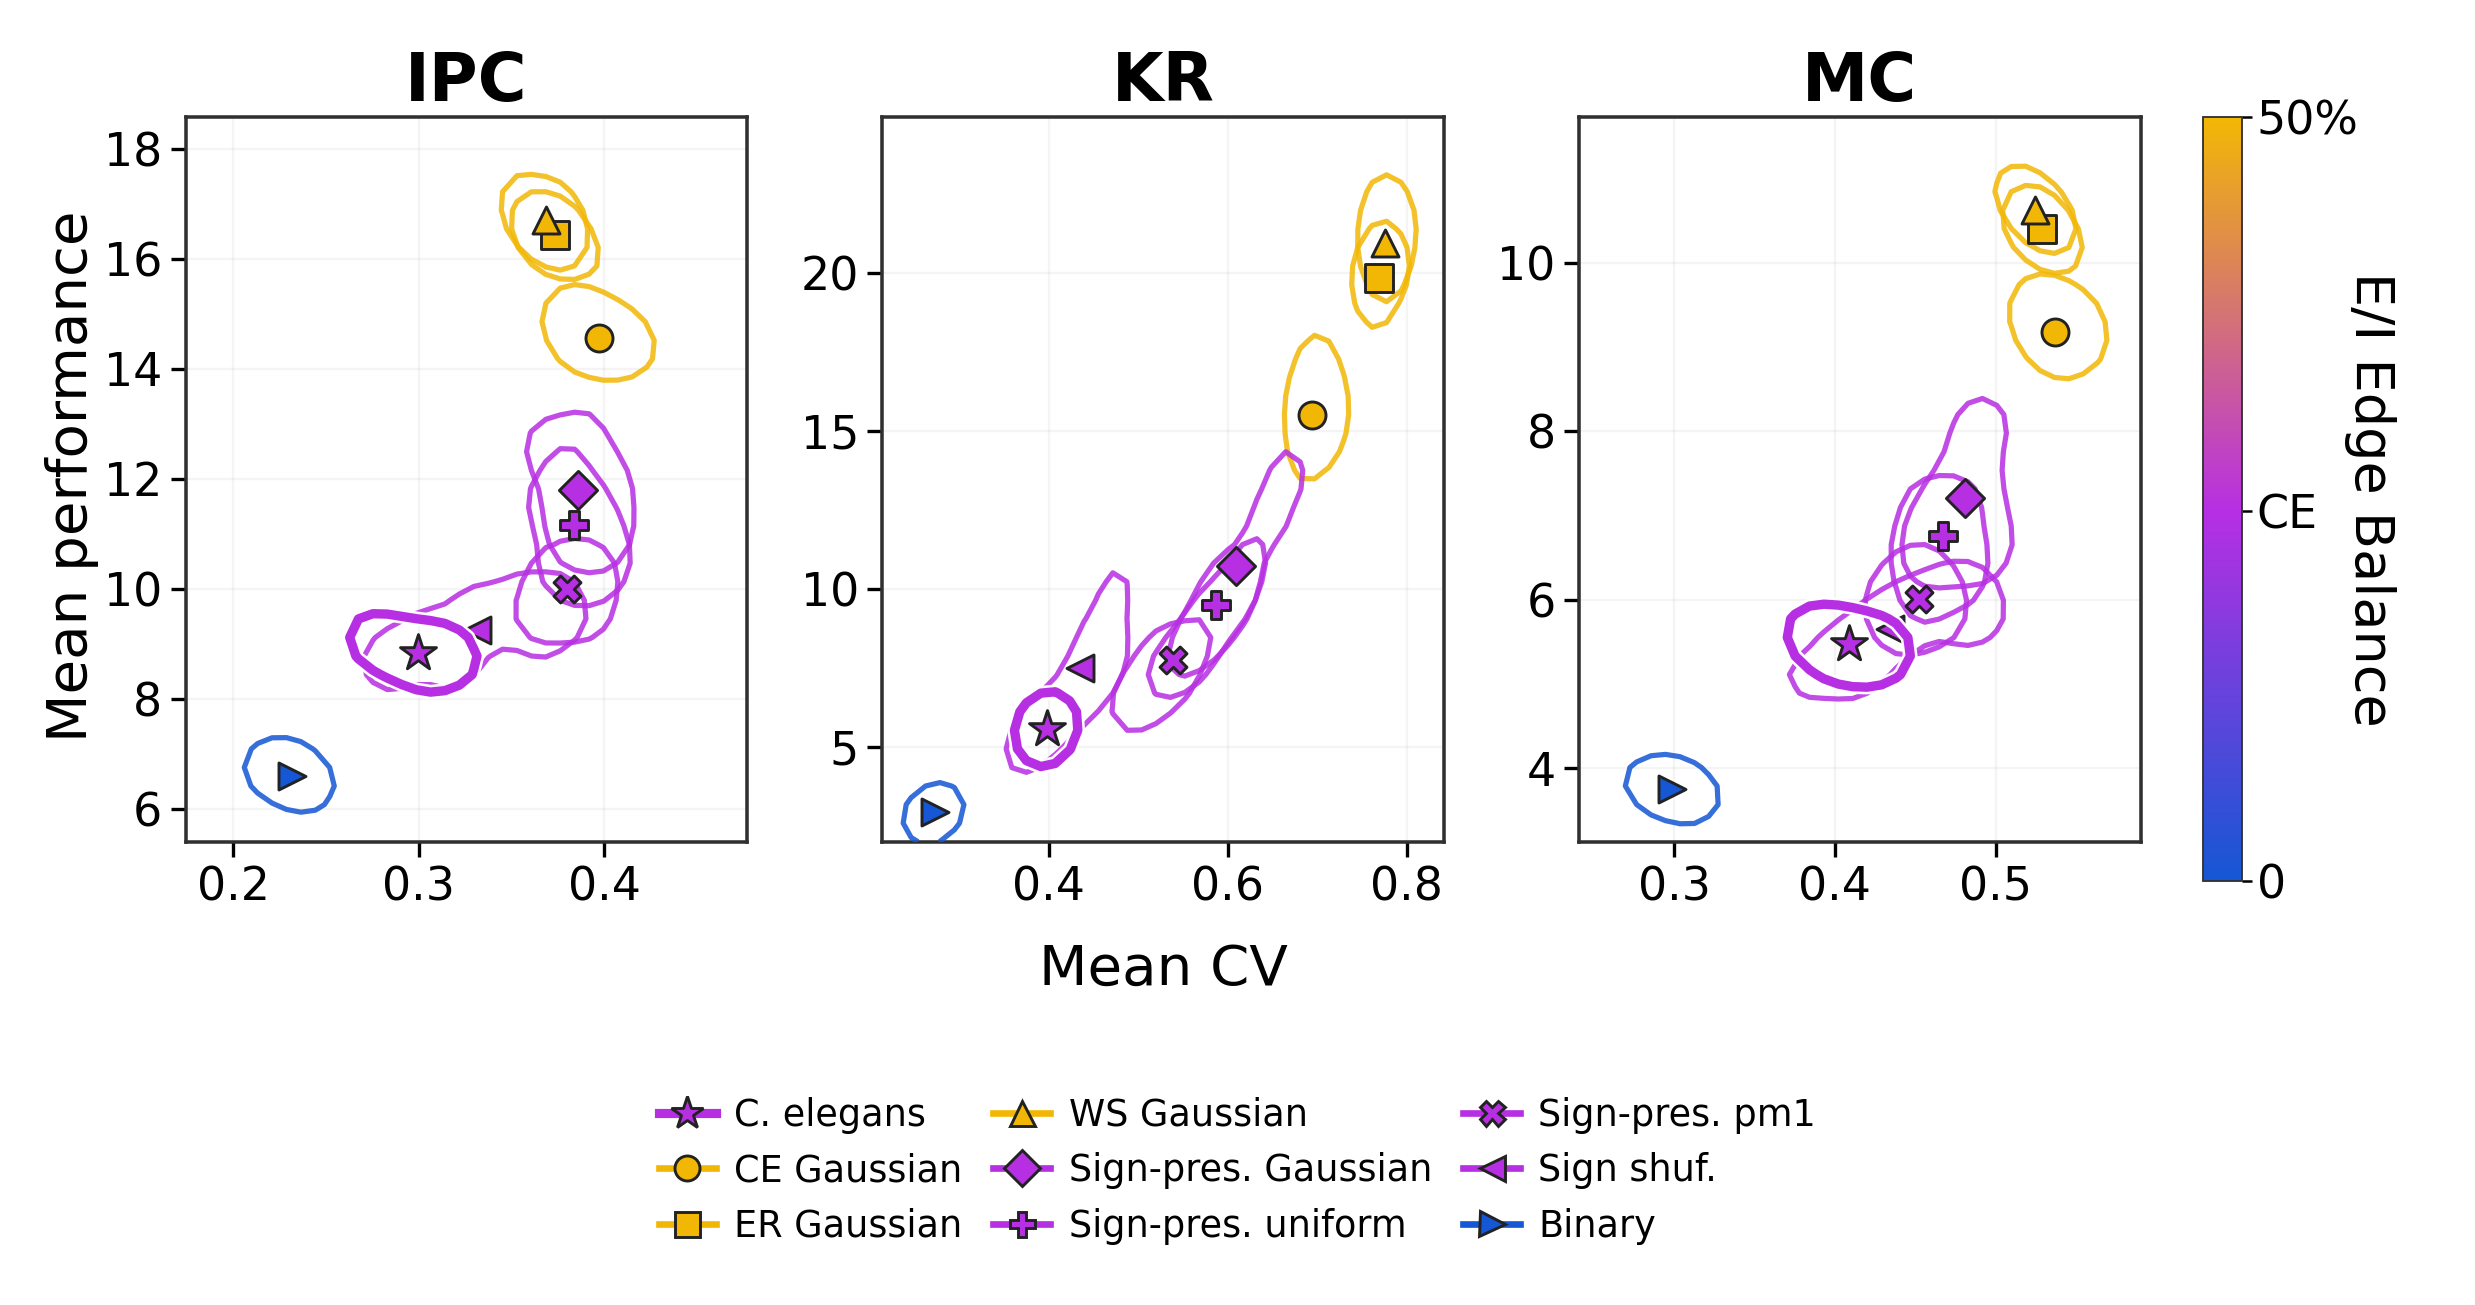
\includegraphics[width=0.76\linewidth]{figures/architecture_tradeoff.png}
\begin{minipage}{0.94\linewidth}
\small\textbf{Figure \thefigure:} Performance--robustness island plots for the architecture comparison. Each panel plots mean task-agnostic performance against hyperparameter CV; contours enclose the highest-density 50\% of trials. Shape identifies architecture and color gives E/I edge balance (blue: 0\% negative edges; purple: empirical \textit{C.~elegans}, approximately 24.25\%; yellow: 50\%). The empirical connectome is the purple star. IPC is the truncated single-delay diagnostic.
\end{minipage}
\end{center}
\medskip

\section{Results}

\paragraph{Architecture comparisons reveal a performance--robustness tradeoff.}
Across IPC, KR, and MC, the architecture families followed a shared positive relationship between mean performance and CV (Figure~\ref{fig:architecture}). Architectures with 50\% negative edges occupied the high-performance, high-CV region, whereas architectures at the empirical E/I edge balance of approximately 24.25\% had lower performance and lower CV. The all-positive binary reservoir occupied the low-performance, low-CV region. Architectures with the same E/I edge balance nevertheless remained separated, showing that topology, sign placement, and weight magnitudes further differentiated performance and robustness.

\paragraph{E/I edge balance sweeps trace the tradeoff.}
When connectivity and weight magnitudes were held fixed, mean IPC, KR, and MC and their CVs were low near the all-positive and all-negative endpoints and increased as the fraction of negative edges approached 50\%. The same pattern was present in the edge-matched random topology and after removing unknown or complex-polarity edges. Across these sweeps, $\rho_{\mathrm{raw}}$ decreased toward 50\% negative edges, so a larger scaling factor was applied near the balanced regime to obtain $W^{\mathrm{res}}$ at the common target radius.

\paragraph{Shuffle controls}
For empirical contact-count weights, degree-preserving connection shuffles, weight shuffles, and their combination increased both mean performance and CV relative to the empirical baseline. With signed-unit weights, sign and connection shuffles instead reduced mean performance and CV.

\paragraph{Generalization rank extends the tradeoff.}
Conditions with higher IPC, KR, and MC also tended to have higher GR. Because lower GR indicates better generalization, increased task-agnostic performance coincided with both greater hyperparameter sensitivity and poorer generalization across input histories. 

\paragraph{Spectral-radius normalization links the experiments.}
Across IPC, KR, and MC, lower raw spectral radius coincided with higher mean performance higher CV and GR, whereas higher raw spectral radius coincided with lower performance, lower CV and GR (Figure~\ref{fig:rawrho}). Higher-performance pertubations showed both greater hyperparameter sensitivity, indicated by higher CV, and reduced generalization, indicated by higher GR. Spectral-radius normalization provides a common framework that unifies these experiments.

\par\medskip
\refstepcounter{figure}\label{fig:rawrho}
\begin{center}
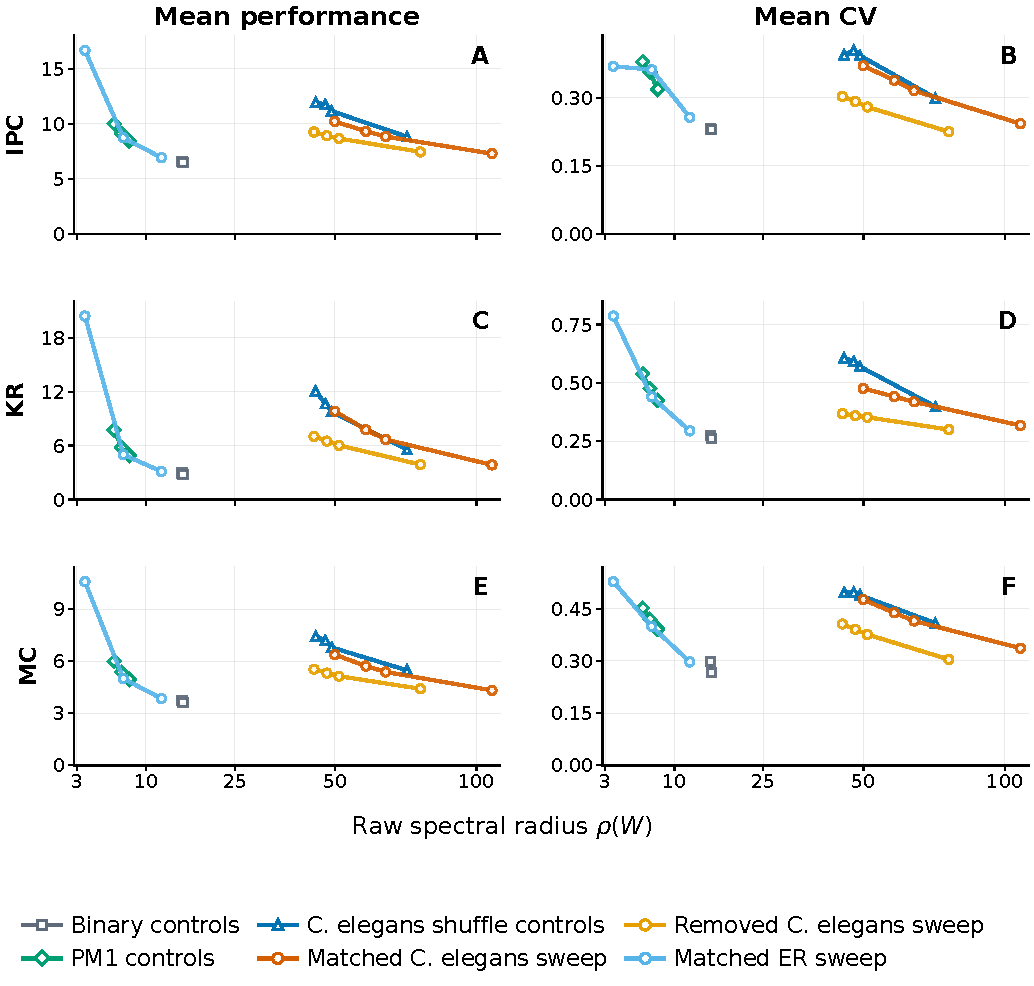
\includegraphics[width=0.49\linewidth]{figures/raw_rho_performance_summary.pdf}
\begin{minipage}{0.92\linewidth}
\small\textbf{Figure \thefigure:} Raw spectral radius and reservoir behavior across the E/I sweeps and shuffle families. Rows show truncated IPC, KR, and MC; columns show mean performance and hyperparameter CV. Lines connect conditions within each experimental family. Across families, lower $\rho_{\mathrm{raw}}$ coincides with higher performance and higher CV under spectral-radius normalization.
\end{minipage}
\end{center}
\medskip

\section{Discussion, Limitations, and NeurReps Relevance}

The empirical \textit{C.~elegans} architecture lies on the low-variance side of a performance--robustness tradeoff rather than near peak task-agnostic performance. Its local topology, sign placement, and weight placement are associated with lower hyperparameter sensitivity and better generalization. Raw spectral radius should therefore be reported in architecture comparisons: it determines the scaling factor used to obtain $W^{\mathrm{res}}$ under standard normalization and changes alongside performance, generalization, and sensitivity, but does not fully explain them \citep{hadaeghi_no_strong_loops_2025}.

Biological interpretation is limited by predicted polarities, unknown or complex edges, omitted electrical synapses, and inputs to all neurons rather than sensory populations. This static reservoir is a structural analysis, not a faithful simulation of the animal. The design cannot isolate the effect of E/I edge balance from its effect on raw spectral radius or from the resulting change in the scaling factor used to obtain $W^{\mathrm{res}}$; more generally, it cannot separate structural changes from their raw-radius consequences.

For NeurReps, the rank analysis connects architecture to representation structure. KR measures effective dimensionality available to separate distinct histories, whereas GR measures dimensions attributable to earlier history after streams share a recent signal. Higher-dimensional, more separable states need not be more invariant or robust: their geometry depends jointly on connectome structure and operating regime. This is a connectome-level account of recurrent separation and generalization without task-specific recurrent training.

\clearpage
\bibliography{references}

\end{document}
